\documentclass[article,A4,12pt]{llncs}
\usepackage[T1]{fontenc}
\usepackage{amsmath}
\usepackage{amssymb}
\usepackage{amsfonts}
\usepackage{mathrsfs, bm}

\usepackage{graphicx}
\usepackage{tabularx}
\usepackage{subfig}
\usepackage{epsf,times}
\usepackage{color}
\usepackage{wrapfig}
\usepackage{cases}
\usepackage{multicol}

\usepackage[T1]{fontenc}
%\newcommand{\tmname}[1]{\textsc{#1}}
%\newcommand{\tmop}[1]{\ensuremath{\operatorname{#1}}}
%\newcommand{\tmsamp}[1]{\textsf{#1}}
%\newcommand{\tmtextsc}[1]{{\scshape{#1}}}
%\newcommand{\tmtextsl}[1]{{\slshape{#1}}}
%\newcommand{\tmtexttt}[1]{{\ttfamily{#1}}}

\leftmargin=0.0cm
\oddsidemargin=0.5cm
\evensidemargin=0.5cm
\topmargin=0cm
\textwidth=16.0cm
%\textheight=21.5cm
\textheight=20.0cm
\pagestyle{plain}
\setlength{\columnsep}{20pt}

\def\m{\mathbf{m}}
\def\H{\mathbf{H}}
\def\E{\mathbf{E}}
\newcommand{\vepsi}{{\varepsilon}}
\def\hnorm#1#2{\vert\,#1\,\vert_{#2}}
\newcommand{\R}{{\mathbb R}}
\newcommand{\Sph}{{\mathbb S}}
\def\x{\mathbf{x}}
\def\hvec{\overline{\mathbf{h}}}
\def\evec{\overline{\mathbf{e}}}

\newcommand{ \etal}{\mbox{\emph{et al. }}}

\newcommand\vect[1]{\mbf{#1}}
\newcommand{\mbf}[1]{\mbox{\boldmath$#1$}} 
\newcommand{\RC}[1]{#1 $\times$ #1 $\times$ #1}
\def\um{$\mu$m}
\def\C{$^{\circ}\mathrm{C}$}

\newcommand{\Rmnum}[1]{\expandafter\@slowromancap\romannumeral #1@}

% DEFINITION OF CUSTOM FONT SIZE
\newcommand{\customfontA}{\fontsize{50}{55}\selectfont}
\newcommand{\customfontB}{\fontsize{14.4}{20}\selectfont}
\newcommand{\customfontC}{\fontsize{30}{35}\selectfont}

\DeclareMathAlphabet{\mathpzc}{OT1}{pzc}{m}{it}

\def\clovek#1{\noindent\bgroup\vbox{\noindent#1}\egroup\vskip1em}

% TO INPUT BACKGROUND IMAGE
\usepackage{eso-pic}
\newcommand\BackgroundPic{
\put(0,0){
\parbox[b][\paperheight]{\paperwidth}{
\vfill
\centering
\includegraphics[width=\paperwidth,height=\paperheight]{img/karel-frontpage.png}
%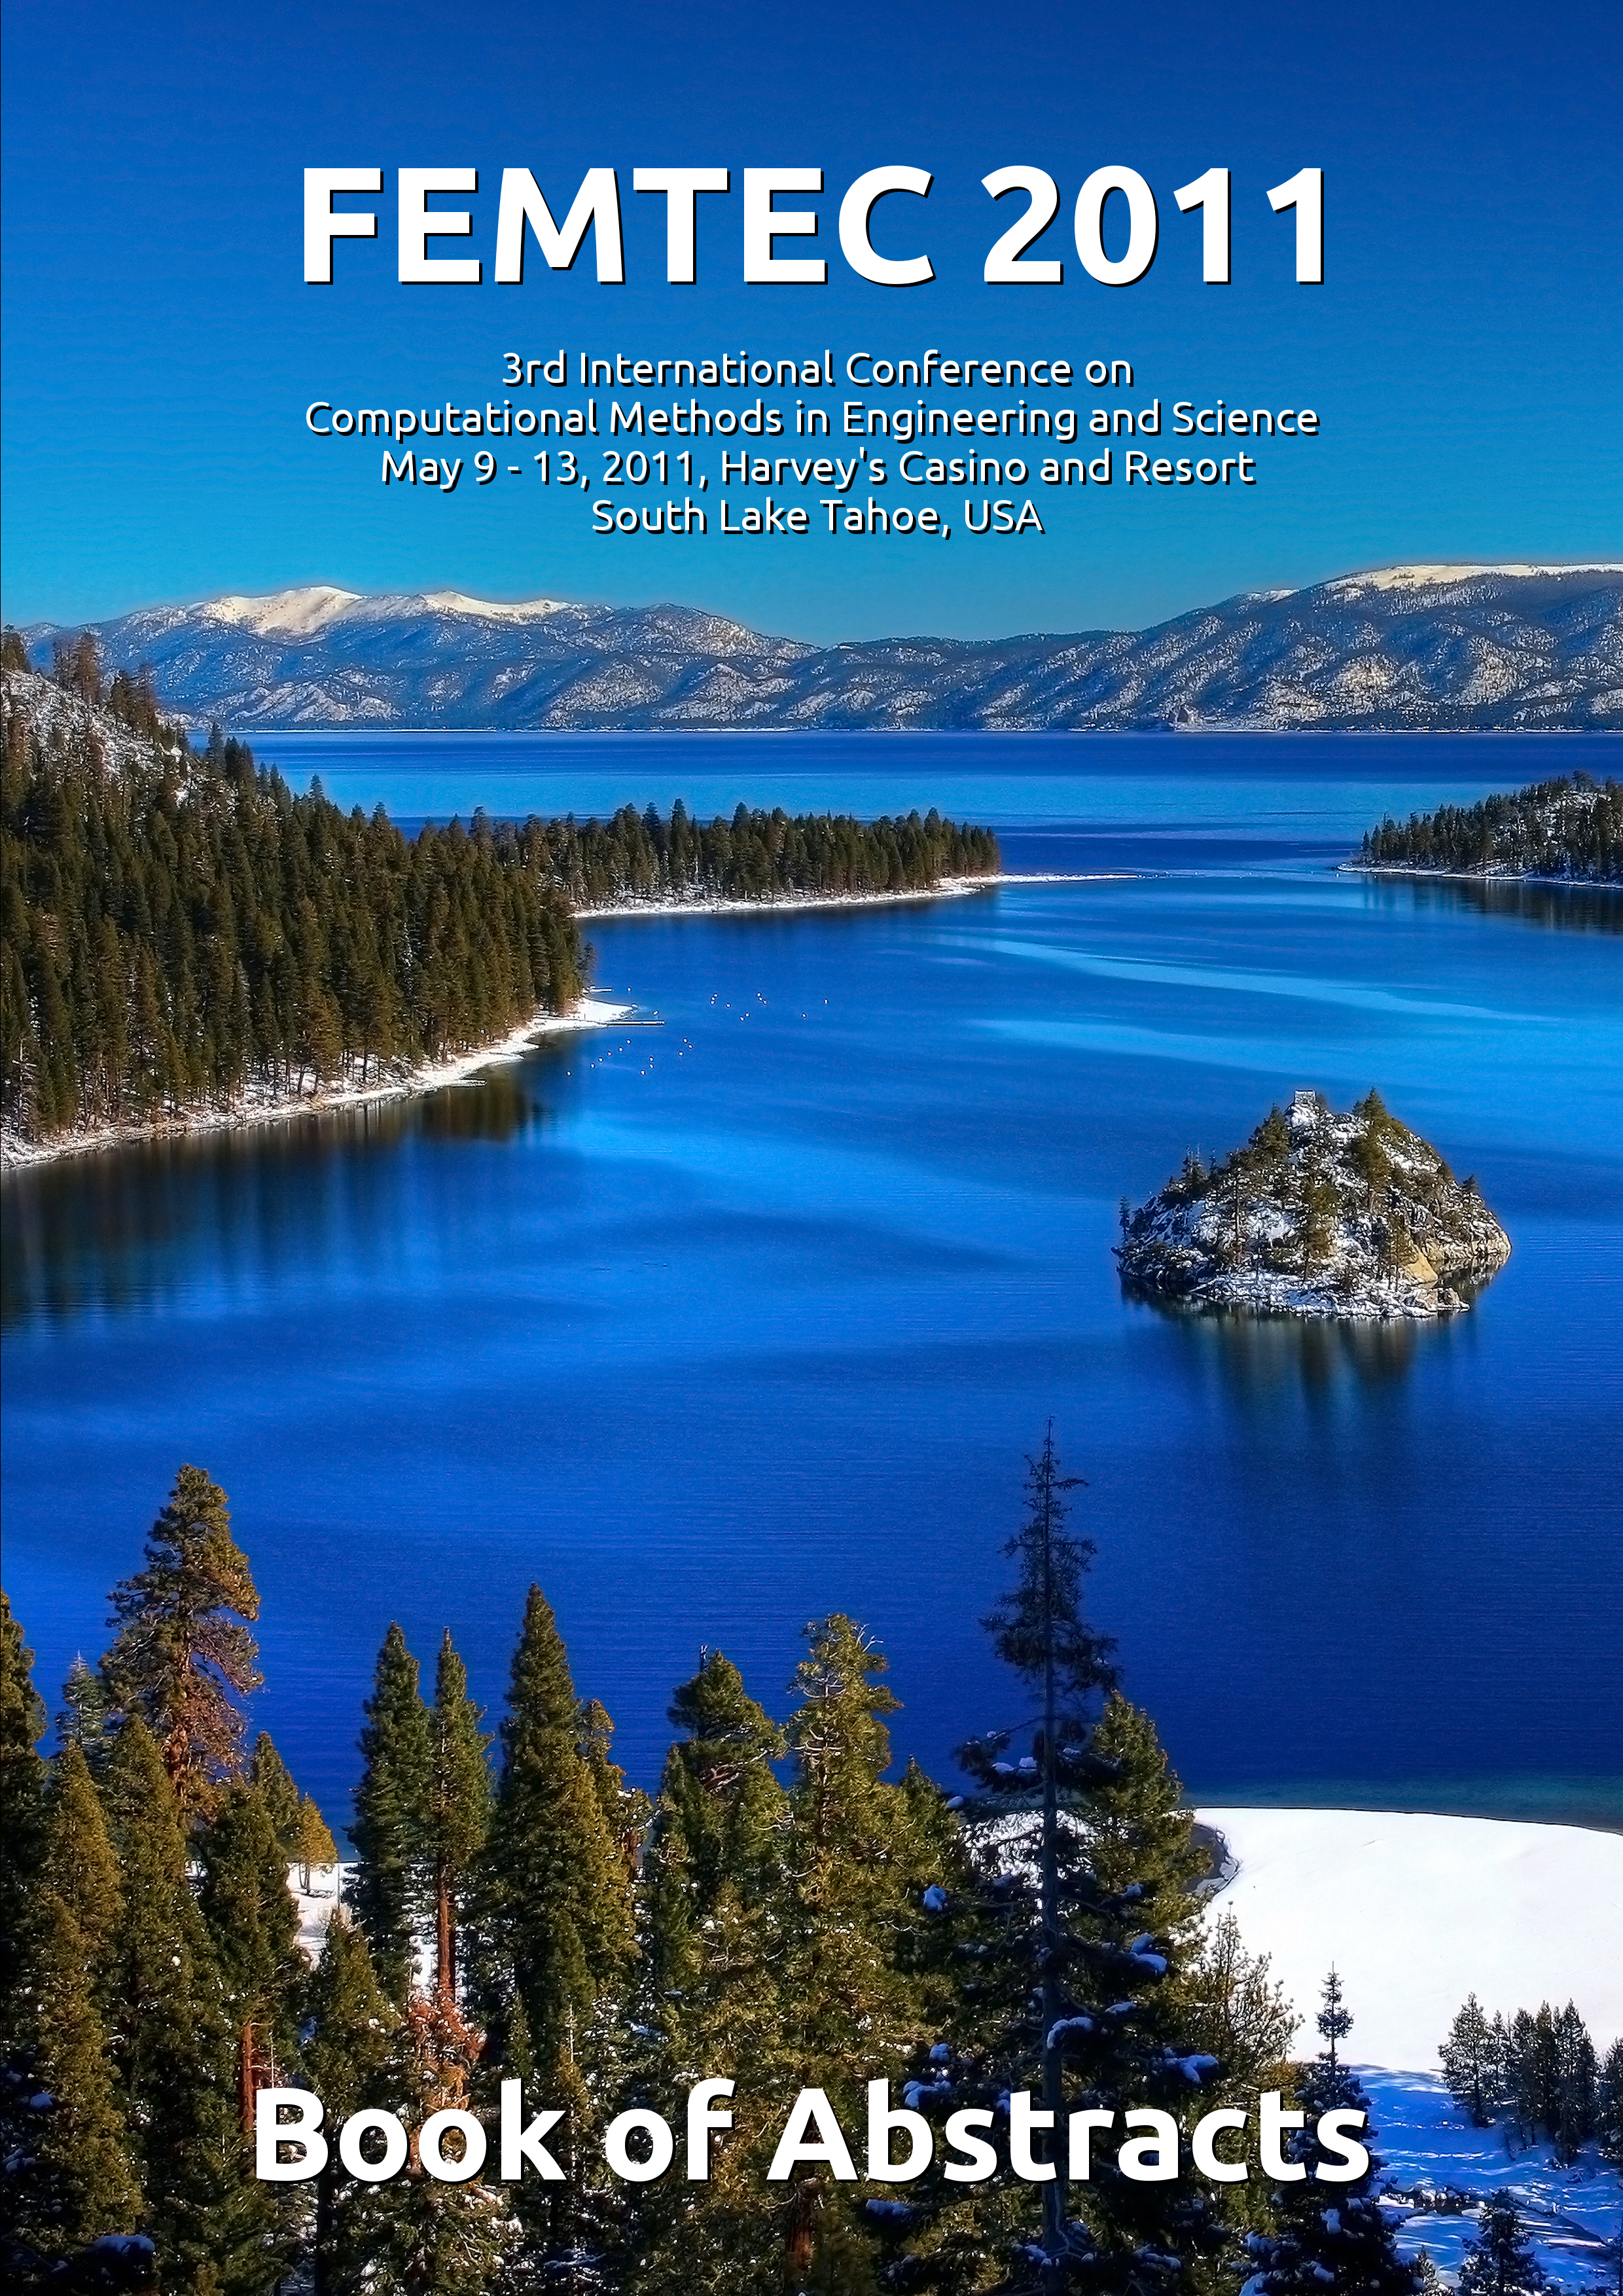
\includegraphics[width=\paperwidth,height=\paperheight]{img/background.jpg}
\vfill
}}}

\begin{document}

% INPUTTING BACKGROUND IMAGE
\AddToShipoutPicture{\BackgroundPic}
\vbox{}
\pagestyle{empty}
\newpage
\textwidth=15.5cm
\ClearShipoutPicture
\newpage

%%%%%%%%%%%%%%%%%%%%%%%%%%%%%%%%%%%%%%%%%%%%%%%%%%%%%%%%%%%%%%%%%%%%%%%%%

\section*{}
\small
\subsection*{About NCLab}
Networked Computing Laboratory (NCLab) is a popular Internet-based framework for 
programming, mathematics, computer modeling, 
and scientific computing. It serves students, instructors, researchers, and the general 
public. NCLab can be used free of charge for personal non-commercial purposes such as 
private hobby or self-education, as well as for individual non-funded academic research.
All other use is subject to {\bf purchasing a license} for a symbolic fee. The fees are as low as 
\$1 per user per month for educational use, and they are used to support the development 
and operational expenses. NCLab is a product of FEMhub Inc. The name "NCLab" is 
registered with the U.S. Patent and Trademark Office (USPTO) under Trademark No. 85420518.

\subsection*{Terms of Use and Pricing}
More details on purchasing a license and using NCLab are provided in the online documents 
{\bf Pricing} and {\bf Terms of Use} that are accessible from NCLab's home page 
{\tt http://nclab.com}.

\subsection*{Contact Information}
General inquiries: {\tt info@femhub.com}\\
Sales: {\tt sales@femhub.com}\\
NCLab support: {\tt support@nclab.com}\\
Agros \& Hermes support: {\tt support@femhub.com}\\
Web page: {\tt http://femhub.com}\\
{Physical address}\\
FEMhub Inc.\\
5490 Twin Creeks Dr.\\
Reno, NV 89523

\subsection*{About This Publication}
This publication can be copied and distributed without any restrictions
as long as reference to NCLab and FEMhub Inc. is preserved.

\subsection*{NCLab's Karel vs. the Original Version}
This publication features {\em Karel the Robot}, a programming language 
designed by Richard E. Pattis. Compared to its original version that was
strongly influenced by Pascal, the NCLab version is closer to Python.
There are some other differences as well that make Karel in NCLab easier to use 
for kids -- Karel collects gems instead of beepers, he has a home in the 
maze, and he uses commands that are much easier for kids to understand
and type. For example, {\tt pickbeeper} was replaced with {\tt get}, 
{\tt front-is-clear} was replaced with {\tt wall}, etc. Even the Python 
colons following every command are omitted because using the SHIFT key 
was causing difficulties to some 5 years old programmers. 
Otherwise we have not changed Pattis' original ideas and all functionality 
covered in Pattis' book is available in the Basic Version of the Programming
module free of charge. 

\normalsize

\newpage
%{\ }
\setcounter{tocdepth}{2}
\tableofcontents
%\pagestyle{plain}

\newpage

\pagestyle{plain}
\setcounter{page}{1}

%%%%%%%%%%%%%%%%%%%%%%%%%%%%%%%%%%%%%%%%%%%%%%%%%%%%%%%%%%%%%%%%%%%%%%%%%

\section{Introduction}

In this introductory course you will learn principles of computer programming with the 
help of an interactive graphical application {\em Karel the Robot} in NCLab. 

\subsection{Brief history}

Karel the Robot is a famous educational programming language that was introduced by Richard E. 
Pattis in his book "Karel The Robot: A Gentle Introduction to the Art of Programming" in 1981. 
Pattis first used the language in his courses at Stanford University, and now it is used at 
countless schools in the world to introduce students to algorithmic design and computer programming. 
The language is named after Karel \v{C}apek, a Czech writer who invented the word "robot" in his 1921 
science fiction play R.U.R. (Rossum's Universal Robots).

\subsection{Who is Karel?}

Karel is a little robot that lives in a maze. The maze contains gems that Karel enjoys to collect. 
He only knows a handful of simple commands such as {\tt go} one step forward, {\tt get} a gem, 
{\tt turn} left, and {\tt put} a gem on the ground. It has built-in sensors that allow him to 
check if a {\tt wall} is in his way, if a {\tt gem} is within his reach, if he is facing {\tt north}, 
if he is at {\tt home}, and if his bag is {\tt empty}. With your help, Karel will learn new things 
that will make it a better Robot, and on the way you will become a Programmer without even noticing! 

\subsection{What is the one reason why I should learn Karel?}

You will learn to {\em design good algorithms} -- an ability that makes
a great programmer and that is completely language-independent. In other 
words, you can learn the same with a technically complicated conventional 
programming language, battling technical problems most of the time,
or you can learn it with Karel the easy way.
Despite its simple form, Karel is not a toy language. It contains all elements 
of a modern procedural programming language. The complexity of algorithms 
covered in this course ranges from {\em very simple} to {\em very tough}.

\subsection{How does Karel differ from conventional programming languages?}

The biggest difference between Karel and all conventional 
programming languages is that it {\em does not involve any mathematics}.
Believe it or not -- Karel does not know numbers. Thanks 
to this, {\em programming concepts} stand out clearly. 
After you finish this tutorial, you will find that suddenly it is very simple 
to learn other languages such as Python or C++, because they are in fact 
very similar to Karel. You will be only learning language-specific details, 
because the most important thing -- algorithmic thinking -- you will already 
know.
 
\section{Getting Started}

In order to make the most of this tutorial, we invite the 
reader to create an account in NCLab and log in. More instructions 
on how to do this are given at the beginning of the introductory 
tutorial "Meet Your New Graphing Calculator" that is available in 
PDF via a link on NCLab home page {\tt http://nclab.com}.\\

\noindent
After logging in, you will see a desktop with several icons on it,
as shown in Fig. \ref{fig:desktop}. 

\begin{figure}[!ht]
\begin{center}
\includegraphics[width=\textwidth]{img/desktop.png}
\end{center}
%\vspace{-2mm}
\caption{NCLab desktop after login.}
\label{fig:desktop}
\end{figure}

\subsection{Launching Karel via the Programming icon}

Karel can be launched in several ways. The simplest one is to click on the icon 
"Programming" and select "Karel" in the menu. This will launch the application 
and load a randomly selected maze, as shown in Fig. \ref{fig:init}.

\begin{figure}[!ht]
\begin{center}
\includegraphics[width=\textwidth]{img/init.png}
\end{center}
%\vspace{-2mm}
\caption{Launching Karel via the Programming icon.}
\label{fig:init}
\end{figure}
\noindent
Karel will be launched in {\em Programming mode} which is the most-frequently 
used mode. You can easily switch to the {\em Manual mode}, {\em Builder},
and {\em Game mode} in the menu. Game mode is available in Full Version only. 
These modes will be discussed in more detail later.

\subsection{Cloning Karel projects} \label{cloning}

All programs and games that we will work with in this course are
available for you to clone (download) into your account. To do this, 
click on the File Manager icon. In the File Manager's menu go to 
"Project" and click on "Clone". This will launch a new window with public
projects as shown in Fig. \ref{fig:cloning}. There are many public
projects to choose from so their loading may take a while. 

\newpage

\begin{figure}[!ht]
\begin{center}
\includegraphics[width=\textwidth]{img/cloning.png}
\end{center}
%\vspace{-2mm}
\caption{Window with public projects is accessible through File Manager's "Project" menu.}
\label{fig:cloning}
\end{figure}
\noindent
All projects that have "Karel" in the Engine column are of interest to you. 
Projects whose names start with "Tutorial - A...", "Tutorial - B..." and 
"Tutorial - C..." are of particular interest. This is done via clicking on the project 
name in the window, and pressing the button "Clone". When you are done, close the 
window. 

In the File Manager's right-hand side panel, you will see the list of all 
projects that you cloned. Click on any of them to launch it. You are free to 
use the cloned projects as they are, or modify them in any way you like. Your modifications 
will not affect the public version of the project. And, you can 
always synchronize your version of the project with the public version, via 
a right-click on the project in the File Manager and selecting "Synchronize".
Beware though -- this will erase any changes that you made to the project.

\subsection{Basic and Full Versions}

If you are using the Programming Module in Basic Version, some restrictions apply: The 
number of projects that you can have at any time is limited to 10, and you cannot have
private projects. Specifically in Karel, the Basic Version does not have the Game mode 
enabled. Besides this, the Basic Version of Karel is fully functional without any other 
limitations. 

If you are logged with an institution code, your Programming module is
probably in Full Version and you should not experience any limitations. If you are 
not logged in with an institution code, you can use the desktop icon "Upgrade" 
to upgrade the Programming module to Full Version.

\subsection{Karel modes}

Karel can operate in four modes:
\begin{itemize}
\item {\em Manual mode:} The robot can be controlled using the mouse and four buttons Go, Get, Turn, and Put. Watch out and do not crash!
\item {\em Program mode:} The robot can be controlled using programs. For simplicity, the Program mode is split into Levels:
\begin{itemize}
\item Level 1 is a transition layer from Manual mode to programming. Programs are written using the commands {\tt go}, {\tt get}, {\tt turn} and {\tt put} that are fully equivalent to pressing the buttons Go, Get, Turn and Put in Manual mode, respectively.
\item Level 2 is where the actual programming begins. On top of the commands from Level 1, programs can contain conditions, loops, and compound commands.
\item Level 3 teaches the user to operate with variables and computer memory. In preparation, available in Full Version only.
\item Level 4 teaches the user basics of object-oriented programming. In preparation, available in Full Version only.
\item Level 5 teaches the user elements of parallel programming. In preparation, available in Full Version only.
\end{itemize}
\item {\em Build mode:} This mode allows the user to create custom worlds for Karel.
\item {\em Game mode:} Makes it possible to create and play games. Available in Full Version only.
\end{itemize}

\section{Lesson One - Beginner}

In the first Lesson you will learn to guide Karel with your mouse.
There are thirteen games that you need to 
solve. Do not skip levels since each one has something new. Each game can 
be cloned as described in Paragraph \ref{cloning} (you need to be using the 
Programming module in Full Version). 
Kids as little as 3 years old were able to do it, so for you it will be a piece 
of cake. Good luck!

\newpage

\subsection{A01 - Go Button}

{\em Karel is returning from a long walk and his batteries are running out. 
Use the buttons on the left to get him home quickly! }

\begin{figure}[!ht]
\begin{center}
\includegraphics[width=0.7\textwidth]{img/a01.png}
\end{center}
\vspace{-4mm}
\caption{In the first game you need to help the robot get home.}
\label{fig:a01}
\end{figure}
\noindent
Pressing Start will start 
the game, and at this time also the buttons Go, Turn, Get and Put appear, 
as shown in Fig. \ref{fig:a01b}.

\begin{figure}[!ht]
\begin{center}
\includegraphics[width=0.7\textwidth]{img/a01b.png}
\end{center}
\vspace{-4mm}
\caption{Karel can be guided manually, using four buttons located in the left panel.}
\label{fig:a01b}
\end{figure}

\newpage

\subsection{A02 - Olympic Games 1980}

{\em Karel is training for Robolympic Games! Your task is to run with 
the robot home as fast as possible. Karel's personal record is four seconds. How fast are you?}

\begin{figure}[!ht]
\begin{center}
\includegraphics[width=0.7\textwidth]{img/a02.png}
\end{center}
\vspace{-4mm}
\caption{Karel is training for Robolympic Games.}
\label{fig:a02}
\vspace{-4mm}
\end{figure}
\noindent

\subsection{A03 - Get Button}

{\em Today is Karel's lucky day because he is about to find his first gem. 
Use the buttons on the left to help the robot pick up the gem and carry it 
home!}

\begin{figure}[!ht]
\begin{center}
\includegraphics[width=0.7\textwidth]{img/a03.png}
\end{center}
\vspace{-4mm}
\caption{Karel is about to find his first gem.}
\label{fig:a03}
\vspace{-1cm}
\end{figure}
\noindent
\newpage

\subsection{A04 - Olympic Games 1984}

{\em It is Robolympic season again! Run home as fast as you can, 
and collect all three gems on the way! Karel's personal record is 10 seconds.}

\begin{figure}[!ht]
\begin{center}
\includegraphics[width=0.7\textwidth]{img/a04.png}
\end{center}
\vspace{-4mm}
\caption{Karel's second Robolympic Games.}
\label{fig:a04}
\end{figure}
\noindent


\subsection{A05 - Turn Button}

{\em Help the robot to collect the gem and return home!}

\begin{figure}[!ht]
\begin{center}
\includegraphics[width=0.7\textwidth]{img/a05.png}
\end{center}
\vspace{-4mm}
\caption{Karel is about to learn how to make a left turn.}
\label{fig:a05}
\vspace{-1cm}
\end{figure}
\noindent
\newpage


\subsection{A06 - Olympic Games 1988 }

{\em Karel is training for his third Robolympic Games. Run with him around the block and home as fast as possible. He needs to collect at least one gem on the way. Karel's personal record is 16 seconds!}

\begin{figure}[!ht]
\begin{center}
\includegraphics[width=0.7\textwidth]{img/a06.png}
\end{center}
\vspace{-4mm}
\caption{Karel's third Robolympic Games.}
\label{fig:a06}
\end{figure}
\noindent


\subsection{A07 - Swirling Tornado}

{\em Pick up the two gems and get Karel home!}

\begin{figure}[!ht]
\begin{center}
\includegraphics[width=0.7\textwidth]{img/a07.png}
\end{center}
\vspace{-4mm}
\caption{Karel will be swirling like a tornado.}
\label{fig:a07}
\vspace{-1cm}
\end{figure}
\noindent
\newpage

\subsection{A08 - Olympic Games 1992}

{\em Last season of Karel's Robolympics Games is here! The 
robot needs to run home as fast as possible and bring one gem. 
Be careful not to crash, this is a tricky level! Karel's personal record is 26 seconds.}\\[-7mm]

\begin{figure}[!ht]
\begin{center}
\includegraphics[width=0.7\textwidth]{img/a08.png}
\end{center}
\vspace{-4mm}
\caption{Karel's fourth Robolympic Games.}
\label{fig:a08}
\vspace{-4mm}
\end{figure}
\noindent


\subsection{A09 - Maze Quest}

{\em This time Karel got seriously lost while looking for his favorite gem. 
Help him to collect the gem and find his way home!}\\[-7mm]

\begin{figure}[!ht]
\begin{center}
\includegraphics[width=0.7\textwidth]{img/a09.png}
\end{center}
\vspace{-4mm}
\caption{Karel got lost while looking for his favorite gem.}
\label{fig:a09}
\vspace{-4mm}
\end{figure}
\noindent
\newpage

\subsection{A10 - Labyrinth}

{\em This is a true labyrinth and your task is to lead Karel 
home. Remember - think first before going anywhere!}

\begin{figure}[!ht]
\begin{center}
\includegraphics[width=0.7\textwidth]{img/a10.png}
\end{center}
\vspace{-4mm}
\caption{Karel needs to find his way home in a labyrinth.}
\label{fig:a10}
\vspace{-4mm}
\end{figure}
\noindent


\subsection{A11 - Diamond Mine}

{\em Karel discovered an abandoned diamond mine. Use the buttons
on the left to collect all gems and get back home in time!}

\begin{figure}[!ht]
\begin{center}
\includegraphics[width=0.7\textwidth]{img/a11.png}
\end{center}
\vspace{-4mm}
\caption{Karel found an abandoned diamond mine.}
\label{fig:a11}
\vspace{-4mm}
\end{figure}
\noindent
\newpage

\subsection{A12 - Gem Harvest}

{\em If gems are piled up, then a number is showing their amount. 
Help Karel collect all gems in this maze and return home!}\\[-7mm]

\begin{figure}[!ht]
\begin{center}
\includegraphics[width=0.7\textwidth]{img/a12.png}
\end{center}
\vspace{-4mm}
\caption{If gems are piled up, then a number is showing their amount.}
\label{fig:a12}
\vspace{-4mm}
\end{figure}
\noindent


\subsection{A13 - Put Button}

{\em Karel has five gems in his bag. Use the buttons on the left to put the gems on the table and 
return home in time!}\\[-7mm]

\begin{figure}[!ht]
\begin{center}
\includegraphics[width=0.7\textwidth]{img/a13.png}
\end{center}
\vspace{-4mm}
\caption{Karel needs to put five gems on the table..}
\label{fig:a13}
\vspace{-4mm}
\end{figure}
\noindent
\newpage

\section{Lesson Two - Taking the Leap}

In this Lesson you will help Karel solve tasks again,
but no longer using the mouse. From now on you will be 
typing commands {\tt go}, {\tt get}, {\tt turn} and {\tt put} 
instead of pressing the buttons Go, Get, Turn and Put. The 
commands do exactly the same things as the corresponding buttons.  
There are only two new rules to remember:
\begin{enumerate} 
\item Type the commands into the input cell on the left, always one command per line.
\item The program is run by clicking on the "Run program" button in the menu, or by clicking 
      on the link "run" under the input cell.
\end{enumerate}
You can clone all projects in this Lesson into your account via the File Manager's Project
menu, same as you did with the games in Lesson 1, and moreover you can clone their solutions. 
Solution manual in PDF is also provided. 

\subsection{B01 - Go Command}

\subsection{B02 - Get Command}

\subsection{B03 - Turn Command}

\subsection{B04 - Put Command}


\section{Lesson Three - Programmer}

In the third Lesson you will help Karel solve tasks again, but 
now with the help of powerful new magical keywords!


\subsection{C01 - Repeat Command}

\subsection{C02 - Repeat Sequence of Commands}

\subsection{C03 - Nested Repeat Commands}

\subsection{C04 - Conditions}

\subsection{C05 - Conditions}

\subsection{C06 - While Command}

\subsection{C07 - While Command}

\subsection{C08 - While Command}

\subsection{C09 - Defining New Commands}



\end{document}
